\documentclass{wccm2024}

\usepackage{graphicx}
\usepackage{amsmath}
\usepackage{amsfonts}
\usepackage{amssymb}
\usepackage{times}
\usepackage{stmaryrd}
\usepackage{subfig}
\usepackage{multirow}
\title{ON THE ITERATIVE SOLUTION OF SADDLE POINT PROBLEMS USING A SYMMETRIC POSITIVE DEFINITE PRECONDITIONER}

\author{PHILIPPE DEVLOO$^{1}$, GIOVANE AVANCINI$^{2}$ AND MARINA MENEGHEL$^{3}$}

\heading{Philippe Devloo, Giovane Avancini and Marina Meneghel}

\address{$^{1}$ State University of Campinas, Faculty of Civil Engineering\\
Av. Albert Einstein, 901 - Cidade Universitária, Campinas - SP, 13083-852\\
phil@unicamp.br
\and
$^{2}$ State University of Campinas, Faculty of Civil Engineering\\
Av. Albert Einstein, 901 - Cidade Universitária, Campinas - SP, 13083-852\\
giovanea@unicamp.br
\and
$^{3}$ State University of Campinas, Faculty of Civil Engineering\\
Av. Albert Einstein, 901 - Cidade Universitária, Campinas - SP, 13083-852\\
m240534@dac.unicamp.br}

\keywords{Iterative method, saddle-point problem, positive-definite preconditioner, H(div) approximation}

\abstract{Saddle point problems frequently appear in many mathematical and engineering applications. Most systems of partial differential equations with constraints give rise to saddle point linear systems. Typical examples include mixed finite element formulations to solve fluid flows and/or elasticity problems under full incompressibility. The inversion of saddle point problems is challenging due to inherent numerical instability in the direct inversion methods. Many direct and iterative methods have been proposed to overcome this challenges, such as the Schur complement and the Uzawa’s method. In the context of mixed finite element for incompressible flows using stable H(div)-L2 spaces for velocity and pressure, we propose an iterative method that can effectively solve a saddle point problem iteratively by summing a small compressibility to the original matrix. The preconditioning matrix is symmetric positive-definite, which allows the usage of Cholesky decomposition and/or CG-like iterative solvers to compute the incremental solution for the velocities unknowns. A procedure to compute the average pressure of each element of the incompressible problem is developed using the unbalanced fluxes caused by the compressibility perturbation. The average is updated during the iterative process as a function of the velocity increment at each iteration.}

\begin{document}
\thispagestyle{empty}

\section{INTRODUCTION}

Saddle point problems frequently appear in many mathematical and engineering applications. Most sets of partial differential equations with constraints give rise to saddle point linear systems. This is the case, for instance, when one uses mixed finite element formulations to solve incompressible problems such as Darcy flows in a porous media, Navier-Stokes flows and elasticity \cite{brezzi2012mixed,duran2019multiscale,brink1996some}.

The numerical solution of saddle point problems is one of the most challenging in numerical analysis for many reasons. This family of matrices often shows poor spectral properties, and indefiniteness due to the null diagonal block related to the constraint equations. The balance between the approximation space and restraint space is delicate and the inversion of the algebraic system of equations can become unstable if terms with large differences are present \cite{bank1989class}. 

On the other hand, numerical inversion of symmetric positive-definite systems are inherently stable: numerical perturbations introduced by round-off will necessarily be attenuated \cite{rohn1994positive}.

A main concern when using iterative methods is to guarantee the convergence within an acceptable number of iterations. Usually, this condition is directly related to the matrix spectral properties. In practice, the strategies to solve a saddle-point problem are divided into two groups - in the first one are the methods that compute the fields in a staggered manner. The most common method in this category is the Uzawa’s method \cite{uzawa1958iterative} and its variations. In the second group are the methods that solve the fields simultaneously \cite{benzi2005numerical}.

In the context of mixed finite element applied to Darcy equations using stable $H(\text{div})$-$L^2$ spaces for flux and pressure, we have been developing an iterative method that can effectively solve a saddle point problem by introducing a small compressibility to the original matrix allowing for the static condensation of pressures. The resulting matrix is symmetric positive-definite, which allows the usage of Cholesky decomposition or CG-like iterative solvers to compute the incremental solution for the velocities or displacement unknowns. The pressure correction is shown to be proportional to the unbalanced force caused by the compressibility perturbation, and can be explicitly updated during the iterative process once the state variable increment is obtained.

\section{DARCY PROBLEM}

Let $\Omega$ be an open domain with Lipschitz boundary $\partial \Omega = \partial\Omega_D \cup \partial\Omega_N$, where $\partial\Omega_D$ and $\partial\Omega_N$ stand for the Dirichlet and Neumann boundaries, respectively. The mixed form of Darcy equations consist of finding the flux $\boldsymbol{\sigma} \in H(\text{div},\Omega)$ and the pressure $p \in L^2(\Omega)$ such that
\vskip -0.3cm
\begin{equation} \label{eq:darcy}
    \begin{split}
        \boldsymbol{\sigma}= -\mathcal{K}\nabla p, \quad \text{in} \quad \Omega, \\
        \nabla \cdot \boldsymbol{\sigma} = f, \quad \text{in} \quad \Omega, \\
        p = p_D, \quad \text{on} \quad \partial\Omega_D, \\
        \boldsymbol{\sigma} \cdot \boldsymbol{n} = g, \quad \text{on} \quad \partial\Omega_N,
    \end{split}
\end{equation}

\noindent where $\mathcal{K}$ is the permeability tensor, $f \in L^2(\Omega)$ is the source term, $u_D \in H^{1/2}(\Omega)$ is the Dirichlet boundary condition, $g \in L^2(\Omega)$ is the Neumann boundary condition and $\mathbf{n}$ is the outward normal vector to $\partial\Omega_N$.

\subsection{Weak statement}

Applying the standard Galerkin method to Eqs. \eqref{eq:darcy}, the weak form of the Darcy problem reads: find $\boldsymbol{\sigma} \in H(\text{div},\Omega)$ and $u \in L^2(\Omega)$ such that for all $\mathbf{w}_{\boldsymbol{\sigma}} \in H(\text{div},\Omega)$ and $w_p \in L^2(\Omega)$:
\vskip -0.3cm
\begin{equation} \label{eq:weak}
    \begin{split}
        \int_{\Omega} \mathcal{K}^{-1}\boldsymbol{\sigma} \cdot \mathbf{w}_{\boldsymbol{\sigma}} \, d\Omega - \int_{\Omega} p \nabla \cdot \mathbf{w}_{\boldsymbol{\sigma}} \, d\Omega = - \int_{\partial\Omega_D} p_D \, ( \mathbf{w}_{\boldsymbol{\sigma}} \cdot \mathbf{n}) \, d\partial\Omega, \\
        \int_{\Omega} \nabla \cdot \boldsymbol{\sigma} \,w_p \, d\Omega = \int_{\Omega} f w_p \, d\Omega.
    \end{split}
\end{equation}

\subsection{Finite element discretization}

The discretization of Eqs. \eqref{eq:weak} is performed using the Finite Element Method \cite{becker1981finite}. We employ an approximation space based on stable $H(\text{div})$-$L^2$ pair which is De Rham compatible \cite{devloo2022efficient,de2013new}. A conformal $\mathcal{T}=\{\Omega_e,e=1, \cdots, n_e \}$ of $\Omega$ in $n_e$ finite elements $\Omega_e$ is defined. Let $\gamma(h,k)$ be a discretization parameter that solely depends on the mesh size $h$ and the polynomial degree $k$, then the finite element spaces are defined as follows:
\vskip -0.3cm
\begin{equation} \label{eq:spaces1}
    \mathbf{V}^\gamma = \{ \boldsymbol{\sigma} \in H(\text{div},\Omega) : \boldsymbol{\sigma}|_{\Omega_e} \in \mathbf{V}(\Omega_e), \forall \Omega_e \in \mathcal{T} \} \text{,}
\end{equation}
\vskip -0.3cm
\begin{equation} \label{eq:spaces2}
    W^\gamma = \{ p \in L^2(\Omega) : p|_{\Omega_e} \in W(\Omega_e), \forall \Omega_e \in \mathcal{T} \} \text{.}
\end{equation}

Rewriting Eqs. \eqref{eq:weak} using the finite element spaces from Eqs. \eqref{eq:spaces1}-\eqref{eq:spaces2}, the discretized problem thus reads: find $\boldsymbol{\sigma}^\gamma \in \mathbf{V}^\gamma$ and $p^\gamma \in W^\gamma$ such that for all $\mathbf{w}_{\boldsymbol{\sigma}}^\gamma \in \mathbf{V}^\gamma$ and $w_p^\gamma \in W^\gamma$:

\begin{equation} \label{eq:discrete}
    \begin{split}
        \sum_{\Omega_e \in \mathcal{T}} \left(\int_{\Omega_e} \mathcal{K}^{-1}\boldsymbol{\sigma}^\gamma \cdot \mathbf{w}_{\boldsymbol{\sigma}}^\gamma \, d\Omega - \int_{\Omega_e} p^\gamma \, \nabla \cdot \mathbf{w}_{\boldsymbol{\sigma}}^\gamma \, d\Omega \right)=- \sum_{\Omega_e \in \partial\Omega_D} \int_{\partial\Omega_e} p_D \ (\mathbf{w}^\gamma_{\boldsymbol{\sigma}} \cdot \mathbf{n}) \, d\partial\Omega, \\
        \sum_{\Omega_e \in \mathcal{T}} \int_{\Omega_e} \nabla \cdot \boldsymbol{\sigma}^\gamma \, w_p^\gamma \, d\Omega = \sum_{\Omega_e \in \mathcal{T}} \int_{\Omega_e} f w_p^\gamma \, d\Omega.
    \end{split}
\end{equation}

\section{ITERATIVE SOLUTION USING A SYMMETRIC POSITIVE-DEFINITE PRECONDITIONER}

Equations \eqref{eq:discrete} can be expressed in matrix form as:
\vskip -0.3cm
\begin{equation} \label{eq:matrixform}
    \begin{bmatrix}
        \mathbf{A} & \mathbf{B} \\
        \mathbf{B}^T & \mathbf{0}
    \end{bmatrix}
    \begin{Bmatrix}
        \boldsymbol{\sigma}^\gamma \\
        \mathbf{p}^\gamma
    \end{Bmatrix}
    =
    \begin{Bmatrix}
        \mathbf{f}^\gamma_{\boldsymbol{\sigma}} \\
        \mathbf{f}^\gamma_{p}
    \end{Bmatrix}, \qquad
    \begin{bmatrix}
        \mathbf{K}
    \end{bmatrix}
    \begin{Bmatrix}
        \mathbf{\boldsymbol{\beta}}
    \end{Bmatrix}
    =
    \begin{Bmatrix}
        \mathbf{f}
    \end{Bmatrix},
\end{equation}

\noindent where matrix $\mathbf{A}$ represents the flux contribution and matrix $\mathbf{B}$ is the divergent operator which plays the role of imposing a constraint to the solution. The right-hand side vectors $\mathbf{f}^\gamma_{\boldsymbol{\sigma}}$ and $\mathbf{f}^\gamma_{p}$ are the Dirichlet contribution and source term, respectively. This latter often is assumed to be zero.

It is worth a discussion about some properties of problem \eqref{eq:matrixform}. Matrix $\mathbf{A}$ is symmetric positive-definite and contains contributions from facet and internal fluxes. The latter ones can be eliminated from the global system by using a static condensation procedure \cite{guyan1965reduction}. Using the element-wise divergence constant approximation space of \cite{devloo2022efficient} results in a single pressure unknown per element. Thus, the global system comprises only facet fluxes and elemental pressures contributions.

Assuming a solution vector $\boldsymbol{\beta}=\{\boldsymbol{\beta}_1, \boldsymbol{\beta}_2\}^T$ such that $\mathbf{B}^T . \boldsymbol{\beta}_1 = \mathbf{0}$ (i.e. $\boldsymbol{\beta}_1 \in Ker\left( \mathbf{B}^T \right)$), then:
\vskip -0.3cm
\begin{equation}
    \{\boldsymbol{\beta}_1, \boldsymbol{\beta}_2\} \cdot \mathbf{K} \cdot 
    \begin{Bmatrix}
        \boldsymbol{\beta}_1 \\
        \boldsymbol{\beta}_2
    \end{Bmatrix}
    = \boldsymbol{\beta}_1^T \cdot \mathbf{A} \cdot \boldsymbol{\beta}_1 > 0
\end{equation}

We propose a modified matrix
\vskip -0.3cm
\begin{equation}
    \mathbf{\Tilde{G}} =
    \begin{bmatrix}
        \mathbf{A} & \mathbf{B} \\
        \mathbf{B}^T & -\mathbf{C}
    \end{bmatrix}
\end{equation}

\noindent where matrix $\mathbf{C}$ is symmetric positive-definite. Once $\mathbf{C}$ plays the role of adding an artificial compressibility to the system, the static condensation procedure can also be applied to eliminate the pressure unknowns:
\vskip -0.3cm
\begin{equation}
    \bar{\mathbf{G}} = \mathbf{A} + \mathbf{B}\mathbf{C}^{-1}\mathbf{B}^T
\end{equation}
\vskip -0.3cm
\begin{equation}
    \bar{\mathbf{f}} = \mathbf{f}^\gamma_{\boldsymbol{\sigma}} + \mathbf{B}\mathbf{C}^{-1}\mathbf{f}^\gamma_{p}
\end{equation}

\noindent where $\bar{\mathbf{G}}$ is also symmetric positive-definite and can be seen as the Schur complement of block $\mathbf{C}$ of matrix $\mathbf{\Tilde{G}}$. 

The proposed iterative method uses matrix $\bar{\mathbf{G}}$ as a preconditioner for matrix $\mathbf{K}$. Given an approximate solution for the flux $\boldsymbol{\sigma}^k$, where $k$ stands for the iteration counter, an updated solution $\boldsymbol{\sigma}^{k+1}$ can be retrieved by doing: first, the residual $\mathbf{r}^{k}$ is computed as:
\begin{equation}
\boldsymbol{\sigma}^0 = \bar{\mathbf{G}}^{-1}\bar{\mathbf{f}}
\end{equation}
\begin{equation}
\mathbf{p}^0 = C^{-1}\left(\mathbf{B}^T \boldsymbol{\sigma}^0-\mathbf{f}_p^\gamma\right)
\end{equation}
\vskip -0.3cm
\begin{equation}
    \mathbf{r}^{k} = - \mathbf{B}\mathbf{C}^{-1}\left(\mathbf{B}^T \boldsymbol{\sigma}^k-\mathbf{f}_p^\gamma \right) .
\end{equation}

\noindent Then, we compute the solution increment:
\vskip -0.3cm
\begin{equation}
    \Delta\boldsymbol{\sigma}^k = \mathbf{\bar{G}}^{-1} \mathbf{r}^{k}
\end{equation}

\begin{equation}
\Delta \mathbf{p}^k = C^{-1}\mathbf{B}^T\Delta \boldsymbol{\sigma}^k
\end{equation}

\noindent finally yielding
\vskip -0.3cm
\begin{equation}
    \boldsymbol{\sigma}^{k+1} = \boldsymbol{\sigma}^{k} + \Delta\boldsymbol{\sigma}^k
\end{equation}
\vskip -0.3cm
\begin{equation}
    \mathbf{p}^{k+1} = \mathbf{p}^{k} + \Delta\mathbf{p}^k
\end{equation}

In engineering terms, the matrix of an incompressible problem is preconditioned by a matrix corresponding to a slightly compressible system. To demonstrate its convergence, we start from the basic description of the iterative method:
\vskip -0.3cm
\begin{equation}
    \Delta\boldsymbol{\beta}^{k} = \boldsymbol{\beta}^{k+1} - \boldsymbol{\beta}^{k} = \mathbf{\Tilde{G}}^{-1} \left( \mathbf{f} - \mathbf{K} \boldsymbol{\beta}^k \right)
\end{equation}
\vskip -0.3cm
\begin{equation}
    \Delta\boldsymbol{\beta}^{k+1} = \boldsymbol{\beta}^{k+2} - \boldsymbol{\beta}^{k+1} = \mathbf{\Tilde{G}}^{-1} \left( \mathbf{f} - \mathbf{K} \boldsymbol{\beta}^{k+1} \right)
\end{equation}

\noindent such that
\vskip -0.3cm
\begin{equation}
    \Delta\boldsymbol{\beta}^{k+1} - \Delta\boldsymbol{\beta}^{k} = \mathbf{\Tilde{G}}^{-1} \mathbf{K} \Delta\boldsymbol{\beta}^{k}
\end{equation}

\noindent or
\vskip -0.3cm
\begin{equation}
    \Delta\boldsymbol{\beta}^{k+1} = \left( \mathbf{I} - \mathbf{\Tilde{G}}^{-1} \mathbf{K} \right) \Delta\boldsymbol{\beta}^{k}
\end{equation}

\noindent which implies that the iterative method will converge if $\left( \mathbf{I} - \mathbf{\Tilde{G}}^{-1} \mathbf{K} \right)$ is a contraction i.e. if its maximum eigenvalue is less than one. One notices that for $\mathbf{\Tilde{G}} = \mathbf{K}$, no solution increment is obtained, so the method converges in a single iteration.

From \cite{gurtin1982introduction}, we can approximate the inverse of $\mathbf{\Tilde{G}}$ as:
\vskip -0.3cm
\begin{equation}
    \mathbf{\Tilde{G}}^{-1} = \mathbf{K}^{-1}-\mathbf{K}^{-1}
    \begin{bmatrix}
        \mathbf{0} && \mathbf{0} \\
        \mathbf{0} && -\mathbf{C}
    \end{bmatrix}
    \mathbf{K}^{-1} + O(\mathbf{C})
\end{equation}

\noindent so neglecting higher order terms yeilds:
\vskip -0.3cm
\begin{equation}
    \left( \mathbf{I} - \mathbf{\Tilde{G}}^{-1} \mathbf{K} \right) \simeq \mathbf{K}^{-1}
    \begin{bmatrix}
        \mathbf{0} && \mathbf{0} \\
        \mathbf{0} && -\mathbf{C}
    \end{bmatrix}
\end{equation}

\noindent demonstrating that the convergence of the iterative method can be controlled by the size of $\mathbf{C}$. For all the examples analyzed, we arbitrarily chose $\mathbf{C}=\alpha \mathbf{I}$, where $\alpha$ refers to the artificial compressibility parameter.

\section{NUMERICAL RESULTS}

In this section, a tridimensional problem is used to assess the performance and stability of the proposed iterative method. In all analyses, convergence is reached when the Euclidian norm of the residual is less than $10^{-9}$, and the maximum number of iterations is set to 50. The solver step is performed with 8 threads on a workstation with an Intel(R) Xeon(R) Gold 6130 2.10GHz CPU.

\subsection{3D Darcy problem}

The computational domain consists on a unit cube $\Omega=(0,1)\times(0,1)\times(0,1)$ and a uniform mesh of hexahedral elements with $k=2$ and characteristic size $h_e=1/n$, where $n=n_x=n_y=n_z$ is the number of elements used in each dimension, starting from $n=5$ up to $n=60$.  The permeability tensor is assumed to be isotropic and unitary, so $\mathcal{K}=\mathbf{I}_3$. The following harmonic solution is adopted for the pressure field:
\vskip -0.3cm
\begin{equation} \label{eq:analytic-pressure}
    p(x,y,z) = \frac{\sin(\pi x) \sin(\pi y) \sinh(\sqrt{2}\pi z)}{\sinh(\sqrt{2}\pi)} \text{.}
\end{equation}

It is straightforward to derive the corresponding flux field from Eq. \eqref{eq:analytic-pressure}. Figure \ref{fig:analytic-solutions} shows the analytic solutions over the domain. Dirichlet boundary conditions are imposed on all the facets.

\begin{figure}[!ht]
    \centering
    \subfloat[]{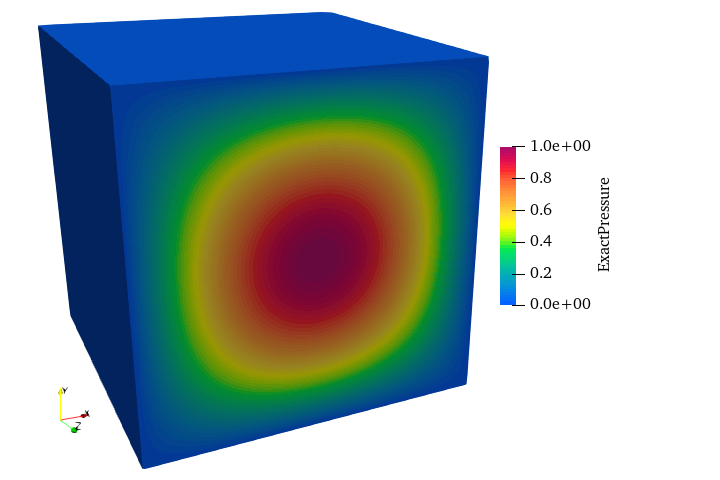
\includegraphics[trim={0cm 0cm 2.42cm 0cm},clip,width=0.49\textwidth]{figs/exact1.png}} \hfill
    \subfloat[]{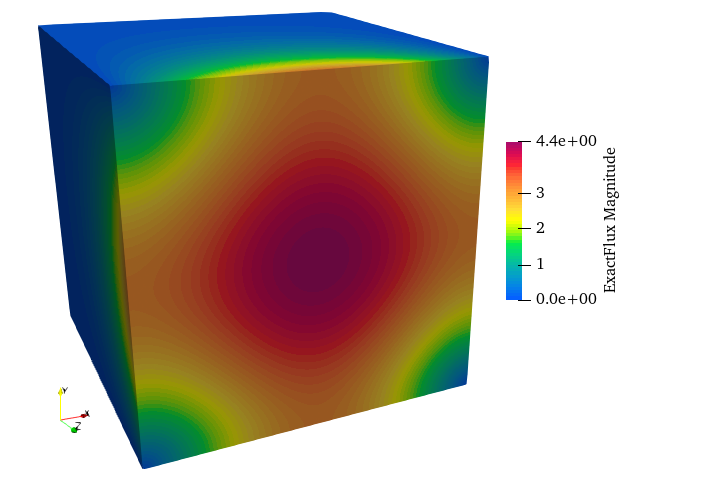
\includegraphics[trim={0cm 0cm 2.42cm 0cm},clip,width=0.49\textwidth]{figs/exact5.png}}
    \caption{3D Darcy problem - analytic solution for the pressure (at left) and flux magnitude (at right).}
    \label{fig:analytic-solutions}
\end{figure}

Firstly, we analyse the convergence of the iterative method as a function of the compressibility parameter $\alpha$. Figure \ref{fig:convergence-alpha} shows the number of iterations required to reach convergence for different values of $\alpha$. It is evident that $\alpha$ plays a key role on the method efficiency, as the higher it gets, the more iterations are required to reach convergence. As the value decreases, we observe a faster convergence as the preconditioner system approximates to the original matrix. However, for excessive small values of $\alpha$, the method shows a loss in the precision. This behaviour is expected as the lower the $\alpha$, the problem tends to the original indefinite saddle-point matrix where Cholesky decomposition likely will fail to find a solution. The optimal value of $\alpha$ also varies with the mesh size. The more refined the mesh, the smaller is the magnitude of the elemental contributions in the global matrix, so the compressibility parameter must be adjusted accordingly.

\begin{figure}[!ht]
    \centering
    \subfloat[$n=10$]{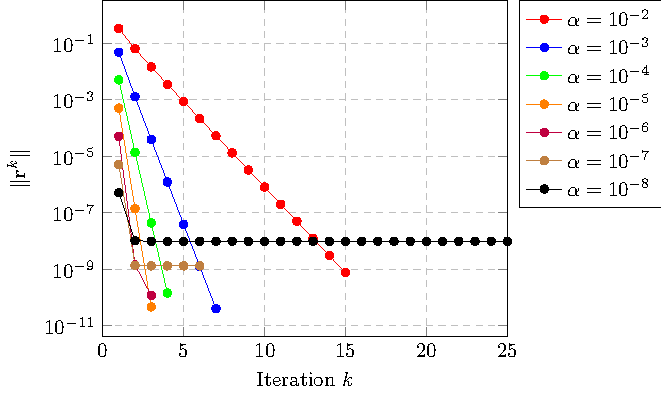
\includegraphics[trim={0cm 0cm 2.42cm 0cm},clip,scale=0.78]{figs/convergence-n-10.pdf}} \hfill
    \subfloat[$n=20$]{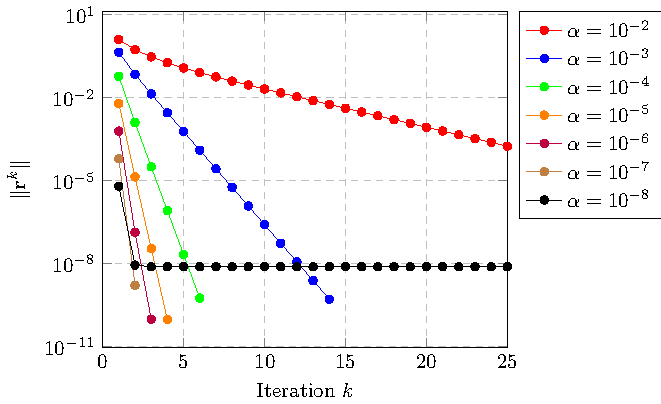
\includegraphics[trim={0cm 0cm 2.42cm 0cm},clip,scale=0.78]{figs/convergence-n-20.pdf}}
    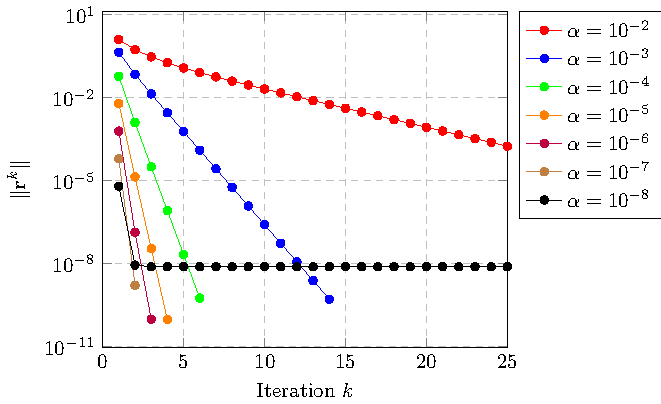
\includegraphics[trim={8.8cm 0cm 0cm 0cm},clip,scale=0.78]{figs/convergence-n-20.pdf} \\
    \subfloat[$n=40$]{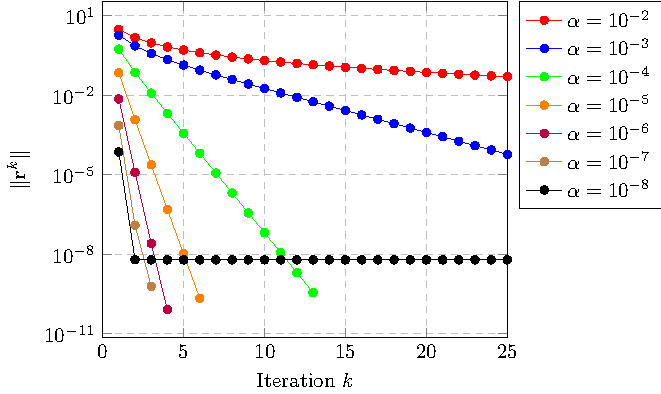
\includegraphics[trim={0cm 0cm 2.42cm 0cm},clip,scale=0.78]{figs/convergence-n-40.pdf}} \hfill
    \subfloat[$n=60$]{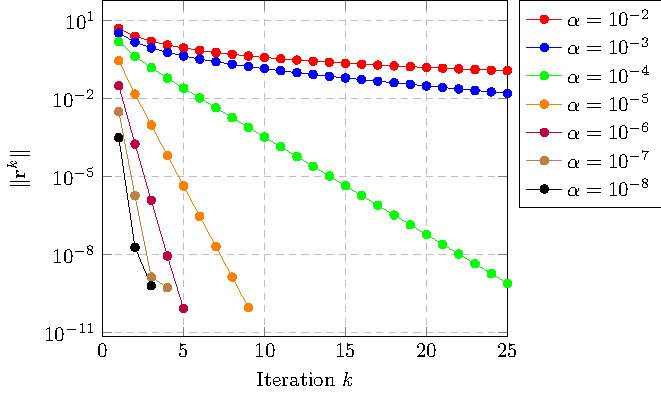
\includegraphics[trim={0cm 0cm 2.42cm 0cm},clip,scale=0.78]{figs/convergence-n-60.pdf}}
    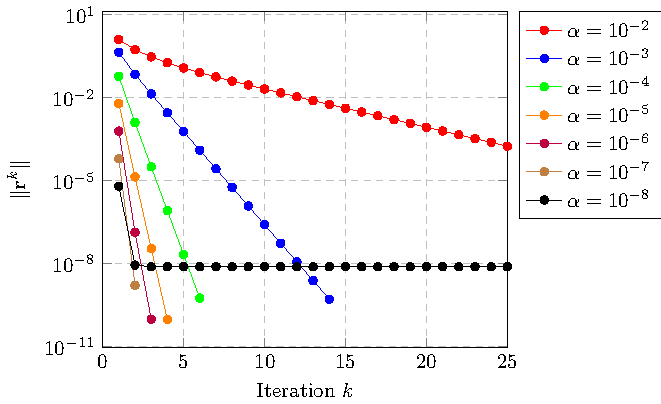
\includegraphics[trim={8.8cm 0cm 0cm 0cm},clip,scale=0.78]{figs/convergence-n-20.pdf}
    \caption{3D Darcy problem - Number of iterations required to reach convergence as a function of the compressibility parameter $\alpha$.}
    \label{fig:convergence-alpha}
\end{figure}

A comparison of the computational cost of the proposed iterative method versus the direct solver is also investigated and displayed in Table \ref{tab:computational-cost}. For these analyses, we use the Cholesky implementation of PARDISO \cite{schenk2000efficient} to build the positive-definite preconditioner for the iterative solver, while the solution of the original saddle-point problem is performed with the LDLT decomposition from PARDISO as well. It shall be highlited that matrix $\mathbf{\Tilde{G}} / \mathbf{C}$ only needs to be decomposed once within the proposed iterative scheme. Thus, the total time is computed as the sum of the time required to build the preconditioner plus the time spent during each iteration solve. The computational cost is presented as a percentage of the time consumed by the direct solver, computed as:
\vskip -0.3cm
\begin{equation}
    \text{Time Consumption [\%]} = \frac{t_{iterative} - t_{direct}}{t_{direct}} \times 100 \text{,}
\end{equation}

\noindent therefore positive values mean that the direct method consumed less time, while negative values indicates a speedup using the proposed iterative method.

\begin{table}[!htb]
    \centering
    \caption{3D Darcy problem - Speedup of the proposed iterative method as a function of the compressibility parameter $\alpha$.}
    \begin{tabular}{ccccccc}
        \hline
        \multirow{2}{*}{Method} & \multicolumn{6}{c}{Time Consumption (\%)}                                \\ \cline{2-7} 
                                & $n=5$ & $n=10$ & $n=20$  & $n=40$   & $n=50$  & $n=60$      \\ \hline
        $\alpha=10^{-2}$        & 66.25   & 99.50    & 396.50 & 406.75 & -        & -           \\
        $\alpha=10^{-3}$        & 32.50   & 42.75    & 68.70  & 85.25 & -        & -           \\
        $\alpha=10^{-4}$        & 21.25    & 20.85    & 17.30  & -3.75 & -3.50 & -11.70 \\
        $\alpha=10^{-5}$        & 25   & 16.35    & 3.80  & -15.60 & -14.80 & -24  \\
        $\alpha=10^{-6}$        & 18.75    & 14    & -2.0  & -23.55 & -21.35 & -27.10 \\
        $\alpha=10^{-7}$        & 71.25   & 33.78    & -2.3  & -25.65 & -23 & -28.10 \\
        $\alpha=10^{-8}$        & -     & -      & -       & -        & -        & -29.50 \\
        % Direct                  & 80    & 379    & 4\,150  & 150\,839 & 540\,429 & 1\,757\,863 \\
        \hline
    \end{tabular}
    \label{tab:computational-cost}
\end{table}

It can be noticed that, for an optimum value of $\alpha$, the iterative method starts to be more efficient than the direct solver for $n \geq 20$. For the finest mesh, a speedup of up to 30 \% can be achieved for $\alpha=10^-8$. However, further studies are needed to determine the optimal value of $\alpha$ as a function of the mesh size. Figure \ref{fig:speedup} shows the time spent during the solution step using the proposed method with the optimum $\alpha$ as a percentage of the time consumed by the direct solver.
\vskip -0.3cm
\begin{figure}
    \centering
    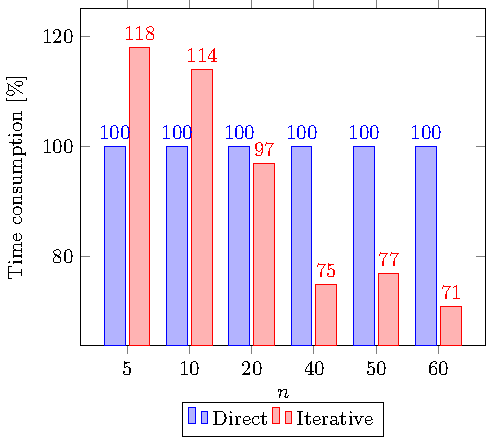
\includegraphics[scale=1.0]{figs/speedup.pdf}
    \caption{3D Darcy problem - Time consumption obtained using the optimum value of $\alpha$ compared to the direct method for different levels of refinement.}
    \label{fig:speedup}
\end{figure}

\section{CONCLUSIONS}

In this work, an iterative method was proposed based on the introduction of a small compressibility to solve saddle point problems using a symmetric positive-definite preconditioner. This scheme not only reduces the number of unkonwns in the global system but also allows the usage of optimized solvers such as Cholesky decomposition and CG-like methods to compute the fluxes increment. The use of an iterative solver to also decompose the preconditioner matrix shall be studied in future works.

The numerical results demonstrated that as the compressibility parameter increases, the number of iterations required to reach convergence also increases. However, for smaller values of $\alpha$, the method converges in less than 3 iterations. Also, an excessive small value of $\alpha$ can lead to numerical instability, as the system becomes ill-conditioned. Therefore, a criterion on how to determine the optimal value of $\alpha$ a priori must be investigated in the future.

As the number of degrees of freedom increases, the proposed method demonstrated to be more efficient than the direct solver. Choosing the apropriate $\alpha$, the computational cost was reduced by up to 30 \% for the most refined mesh.

\vspace{20pt}
\noindent \textbf{Acknowledgements.} We gratefully acknowledge the support of EPIC - Energy Production Innovation Center through FAPESP/Equinor (Grant 2023/06981/-5),  Total Energies Brazil through FUNCAMP (Process 76042-23) and the Brazilian National Council for Scientific and Technological Development (grants 305823/2017-5 and 309597/2021-8). We also acknowledge the support of ANP (Brazil’s National Oil, Natural Gas and Biofuels Agency).
\vspace{12pt}

\bibliographystyle{ieeetr}
\bibliography{references}



\end{document}


